\section{Helpfulness Prediction}
Our ambitious objective was to build a model capable of predicting the helpfulness of a review based solely on the review text.
To create such a model, we first needed to convert the text into a machine-readable format, a process known as \textit{feature extraction}.
Subsequently, we explored different models to identify the one best suited for our needs, ultimately selecting the most appropriate one.

\subsection*{Feature Extraction}
Given the complexity of the problem, we opted to employ a \textit{Word Embedding} technique called \textit{Word2Vec}, which converts words into
vectors of real numbers while preserving their semantic meaning. We utilized the \textit{Gensim} library to perform this task, using the
following parameters for the model:
\begin{itemize}[noitemsep, leftmargin=*]
    \item \textbf{Size}: 30 and 150
    \item \textbf{Window}: 5
    \item \textbf{Min Count}: 2
    \item \textbf{Workers}: -1
\end{itemize}
Consequently, each word is represented by a 30 (or 150) dimensional vector, and the average of these vectors for all words in a review forms the vector
representation of the review.

\subsection*{Models}
We evaluated three different models:\textit{Random Forest},\textit{Support Vector Regressor (RBF kernel)}, and\textit{Multi-Layer Perceptron (MLP)}.
We employed the\textit{Scikit-Learn} library for model training and testing, utilizing the \textit{GridSearchCV} class to perform cross-validation on
the training set to identify the best model parameters. The results are presented in Table \ref{tab:model_results} and visualized in Figure
\ref{fig:model_results}.

\begin{table}[H]
    \footnotesize
    \centering
    \caption{Model Results}
    \label{tab:model_results}
    \begin{tabular}{|c|c|c|c|}
        \hline
        Model & MSE    & RMSE   & R\textsuperscript{2} \\
        \hline
        RF    & 0.0259 & 0.1609 & 0.2532               \\
        SVR   & 0.0279 & 0.1670 & 0.1955               \\
        MLP   & 0.0282 & 0.1680 & 0.1858               \\
        \hline
    \end{tabular}
\end{table}

\begin{figure}[H]
    \centering
    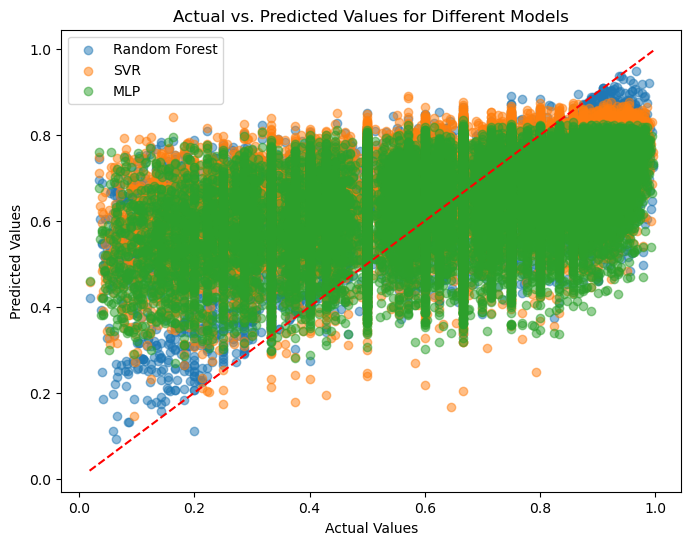
\includegraphics[width=0.35\textwidth]{./figures/model_results.png}
    \caption{Model Results}
    \label{fig:model_results}
\end{figure}

\noindent
The results and metrics used indicate that the \textit{Random Forest} model outperforms the others in terms of Mean Squared Error (MSE)
and Root Mean Squared Error (RMSE). The Random Forest model achieved the lowest MSE of approximately 0.026 and RMSE of approximately 0.161,
suggesting that its predictions are the closest, on average, to the actual values. This implies that the Random Forest model offers the
best overall predictive performance among the three models. To further enhance model performance, we experimented with increasing the
number of features from 30 to 150. However, the performance improvement was not substantial, so we chose to retain 30 features due to the
optimal balance between performance and computational cost.

\subsection*{Results Interpretation}
Figures \ref{fig:model_best_scatter} and \ref{fig:model_best_lines} aid in interpreting the results. The scatter plot visually represents
the distribution of errors, revealing that the model tends to overestimate the helpfulness of reviews with high helpfulness scores and
underestimate those with low scores. A comprehensive analysis of the underlying causes of this behavior, particularly focused on the
feature engineering process, remains a subject for future investigation.

\begin{figure}[H]
    \centering
    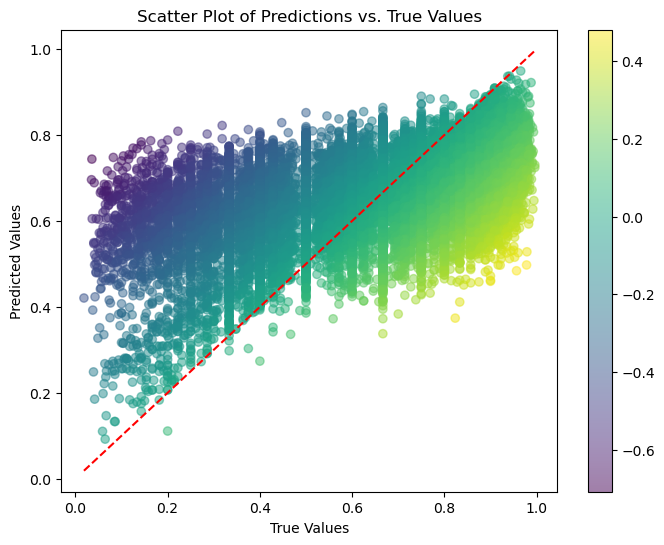
\includegraphics[width=0.35\textwidth]{./figures/model_best_scatter.png}
    \caption{Errors of the Best Model}
    \label{fig:model_best_scatter}
\end{figure}

\noindent
The line plot, on the other hand, provides insights into the meaning of a given helpfulness score by translating it into Total
Votes and Helpfulness Votes. The blue line represents the values (Total Votes, Helpfulness Votes) corresponding to a helpfulness
score close to 0.8, while the red and green lines represent values corresponding to a helpfulness score of 0.8 plus or minus the RMSE.
For instance, for a base of 100 Total Votes, the RMSE of our model corresponds to an excess or deficit of approximately 13 votes.

\begin{figure}[H]
    \centering
    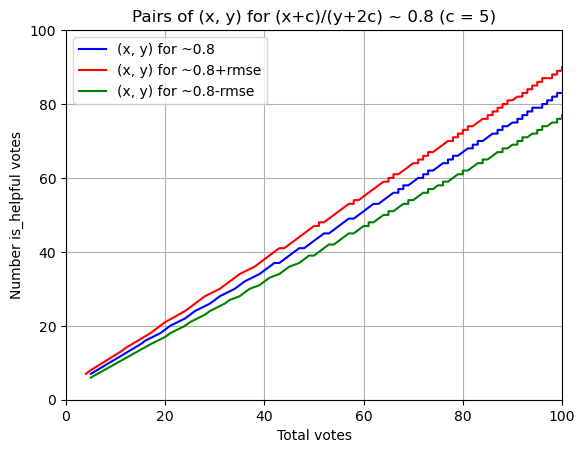
\includegraphics[width=0.3\textwidth]{./figures/model_best_lines.png}
    \caption{Translation of Helpfulness Score Errors}
    \label{fig:model_best_lines}
\end{figure}





